% -*- root: main.tex -*-

\usepackage[pdftex,
            pdfauthor={Eric Peterson},
            pdftitle={Formal Geometry and Bordism Operations}]{hyperref}

\usepackage{fullpage}
% \usepackage{savetrees}
\usepackage{amsmath,amssymb,amsthm}
\usepackage{stmaryrd} % for \llbracket and \rrbracket
\usepackage[version warn]{sseqpages/sseqpages}

% \usepackage[urw-garamond]{mathdesign}
\usepackage{mathpazo} % math & rm
\linespread{1.05}        % Palatino needs more leading (space between lines)
\usepackage[scaled]{helvet} % ss
\usepackage{courier} % tt
\normalfont
\usepackage[T1]{fontenc}

\usepackage{tikz}
\usetikzlibrary{matrix,calc,3d,arrows,positioning,fadings}

\usepackage{tikz-cd}
\makeatletter
\tikzcdset{
    iso/.style="\cong"{#1},
    iso'/.style="\cong"{/utils/exec=\isop@which,#1},
    equiv/.style="\simeq"{#1},
    equiv'/.style="\simeq"{/utils/exec=\isop@which,#1},
    equal/.style={double distance=2pt,-}
}

\def\isop@getrow#1-#2-#3\@nil{#2}
\def\isop@getcolumn#1-#2-#3\@nil{#3}
\def\isop@which{
    \ifnum\@xp\isop@getrow\tikzcd@ar@start\@nil=\@xp\isop@getrow\tikzcd@ar@target\@nil\relax
        \pgfkeysalso{yscale=-1}
        \ifnum\@xp\isop@getcolumn\tikzcd@ar@start\@nil>\@xp\isop@getcolumn\tikzcd@ar@target\@nil\relax
            \pgfkeysalso{'}
        \fi
    \else
        \pgfkeysalso{'}
    \fi
}
\makeatother


\usepackage[textsize=tiny]{todonotes}
\usepackage[missing={See gitinfo2 instructions},dirty={(*)}]{gitinfo2}

\usepackage{pdflscape}
\usepackage[figuresright]{rotating}
\usepackage{mathtools}

% used for \bigast
\usepackage{relsize}

% make the bibliography appear in the table of contents
\usepackage[nottoc,numbib]{tocbibind}

\usepackage{cleveref}

% used to set custom chapter titles
\usepackage{tocloft,calc}

% this steals from http://tex.stackexchange.com/questions/36006/how-can-i-use-a-symbol-provided-by-a-package-without-changing-the-entire-mathema to import the "action" arrow
\DeclareFontFamily{U} {MnSymbolA}{}

\DeclareFontShape{U}{MnSymbolA}{m}{n}{
  <-6> MnSymbolA5
  <6-7> MnSymbolA6
  <7-8> MnSymbolA7
  <8-9> MnSymbolA8
  <9-10> MnSymbolA9
  <10-12> MnSymbolA10
  <12-> MnSymbolA12}{}
\DeclareFontShape{U}{MnSymbolA}{b}{n}{
  <-6> MnSymbolA-Bold5
  <6-7> MnSymbolA-Bold6
  <7-8> MnSymbolA-Bold7
  <8-9> MnSymbolA-Bold8
  <9-10> MnSymbolA-Bold9
  <10-12> MnSymbolA-Bold10
  <12-> MnSymbolA-Bold12}{}
\DeclareSymbolFont{MnSyA} {U} {MnSymbolA}{m}{n}
% 184 and 255 are both good options
\DeclareMathSymbol{\actson}{\mathrel}{MnSyA}{255}


%%% DONE WITH PACKAGES

\setlength{\marginparwidth}{1in-\marginparsep} % fullpage sets margins to 1in

% todonotes definitions

\newcommand{\oweproof}[1]{\todo[color=red]{\textbf{You owe a proof of: } #1.}}
\newcommand{\citeme}[1]{\todo[color=green]{\textbf{Cite me: } #1.}}
\newcommand{\needproof}[1]{\todo[color=magenta]{\textbf{I need to already know: } #1.}}


% symbol definitions

% -*- root: main.tex -*-

% this macro was written by Hood Chatham, May 2016

\makeatletter
\def\makesymbdefs#1#2{\setcharsuff{#2}{#1}{abcdefghijklmnopqrstuvwxyzABCDEFGHIJKLMNOPQRSTUVWXYZ}}
\let\@xp\expandafter
\newtoks\setchars@toks
\def\setchars#1#2{\def\setchar@name##1{##1}\setchars@{#1}{#2}}
\def\setcharsuff#1#2#3{\def\setchar@name##1{##1#2}\setchars@{#1}{#3}}
\def\setchars@#1#2{\setchars@toks{\setchars@@{#1}}\edef\next{\the\setchars@toks#2.}\next}
\def\setchars@@#1#2{
    \ifx#2.\else
        \def\temp##1{#1}
        \setchars@usedparam\temp % If you delete optional block, delete this line too
        \@xp\def\csname\setchar@name{#2}\@xp\endcsname\@xp{\@xp{\temp{#2}}}
        \setchars@toks{\setchars@@{#1}}
        \@xp\the\@xp\setchars@toks
    \fi
}

%optional
\bgroup\lccode`*=`#\lowercase{\egroup
    \def\setchars@usedparam#1{
        \@xp\setchars@usedparam@\@xp#1\meaning#1*\@nil
    }
    \def\setchars@usedparam@#1#2->#3*#4\@nil{
        \ifx&#4&
            \@xp\def\@xp#1\@xp{#1{}}
        \fi
    }
}
%end optional
\makeatother


% Use cases: 
% \setchars{\mathbb}{NZQRC} % (or \setchars{\mathbb{#1}}{NZQRC} **)
% \setchars{\mathcal}{O}  % (or \setchars{\mathcal{#1}}{O} **)
% \setchars{\widehat{\mathbb{#1}}}{AG}
% \makesymbdefs{bb}{\mathbb} % Defines \Abb, \Bbb, \Cbb, etc to expand to \mathbb{A}, etc
% \makesymbdefs{x}{#1^{\times}}


\setchars{\mathbb}{NZQRCSFPWH} % (or \setchars{\mathbb{#1}}{NZQRC} **)
\setchars{\mathcal}{LHO}  % (or \setchars{\mathcal{#1}}{O} **)
\setchars{\widehat{\mathbb{#1}}}{AG}
\setchars{\mathfrak}{mhp}

\newcommand{\barG}{\overline{\mathbb G}}
\newcommand{\RP}{\R\mathrm P}
\newcommand{\CP}{\C\mathrm P}
\newcommand{\HP}{\mathbb H\mathrm P}
\newcommand{\FH}{\textbf{FH}}
\newcommand{\CH}{\textbf{CH}}
\renewcommand{\t}{\mathbf t}
\newcommand{\Gm}{\mathbb G_m}
\newcommand{\ThomDivisor}{\mathbb D}

\newcommand{\<}{\langle}
\renewcommand{\>}{\rangle}
\newcommand{\sm}{\wedge}
\newcommand{\Susp}{\Sigma}
\newcommand{\Loops}{\Omega}
\renewcommand{\phi}{\varphi}
\renewcommand{\epsilon}{\varepsilon}
\newcommand{\eps}{\varepsilon}
\newcommand{\mmod}{/\!\!/}
\newcommand{\co}{\colon\thinspace}
\newcommand{\into}{\hookrightarrow}
\newcommand{\cotensor}{\square}
\newcommand{\from}{\leftarrow}
\newcommand{\onto}{\twoheadrightarrow}
\newcommand{\mhyphen}{\text{-}}
\newcommand{\adjunct}[4]{{#1}\colon\thinspace{#2} 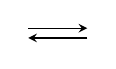
\begin{tikzpicture}[baseline] \draw[>=stealth,->] (0,1ex) -- (0.75,1ex); \draw[>=stealth,->] (0.75,0.25ex) -- (0,0.25ex); \end{tikzpicture}\ {#3}\thinspace\colon{#4}}

\renewcommand{\th}{\textsuperscript{th}}
\newcommand{\st}{\textsuperscript{st}}
\def\Cech{\v{C}ech}

\newcommand{\bigast}{\mathop{\vcenter{\hbox{$\mathlarger{\mathlarger{\ast}}$}}}}

\newcommand{\context}[1]{\mathcal{M}_{#1}}
\newcommand{\Ucontext}[1]{\mathcal{UM}_{#1}}
\newcommand{\CatOf}[1]{\mathsf{#1}}
\newcommand{\ps}[1]{\llbracket{#1}\rrbracket}
\newcommand{\moduli}[1]{\mathcal{M}_{\mathbf{#1}}}
\newcommand{\OS}[2]{\underline{\smash{#1}}_{#2}}
\newcommand{\InternalHom}[1]{\operatorname{\underline{\smash{\CatOf{#1}}}}}
\newcommand{\InternalAut}{\operatorname{\underline{\smash{\operatorname{Aut}}}}}
\newcommand{\InternalEnd}{\operatorname{\underline{\smash{\operatorname{End}}}}}
\newcommand{\sheaf}[1]{\mathcal{#1}}
\newcommand{\ThomSheaf}[1]{\mathbb{L}(#1)}

\newcommand{\Spin}{\mathit{Spin}}
\newcommand{\String}{\mathit{String}}
\newcommand{\TMF}{\mathit{TMF}}
\newcommand{\Tmf}{\mathit{Tmf}}
\newcommand{\tmf}{\mathit{tmf}}
\newcommand{\TAF}{\mathit{TAF}}
\newcommand{\BP}{\mathit{BP}}
\newcommand{\MU}{\mathit{MU}}
\newcommand{\Tate}{\mathrm{Tate}}
\newcommand{\gl}{\mathit{gl}}
\newcommand{\GL}{\mathit{GL}}
\newcommand{\perf}{\mathrm{perf}}
\newcommand{\gpd}{\mathrm{gpd}}
\newcommand{\ptyp}{p\text{-}\mathrm{typ}}
\newcommand{\id}{\mathrm{id}}
\newcommand{\FGps}{\mathrm{FGps}}
\newcommand{\fin}{\mathrm{fin}}

\DeclareMathOperator{\Ind}{Ind}
\DeclareMathOperator{\Spec}{Spec}
\DeclareMathOperator{\Spf}{Spf}
\DeclareMathOperator{\Sch}{Sch}
\DeclareMathOperator*{\colim}{colim}
\DeclareMathOperator{\End}{End}
\DeclareMathOperator{\Div}{Div}
\DeclareMathOperator{\SDiv}{SDiv}
\DeclareMathOperator{\Sq}{Sq}
\DeclareMathOperator{\Sym}{Sym}
\DeclareMathOperator{\Aut}{Aut}
\DeclareMathOperator{\Def}{Def}
\DeclareMathOperator{\Pic}{Pic}
\DeclareMathOperator{\Ext}{Ext}
\DeclareMathOperator{\hAut}{hAut}
\DeclareMathOperator{\Coord}{Coord}
\DeclareMathOperator{\Tor}{Tor}
\DeclareMathOperator{\Cotor}{Cotor}
\DeclareMathOperator{\coker}{coker}
\DeclareMathOperator{\Hom}{Hom}
\DeclareMathOperator{\Weil}{Weil}
\DeclareMathOperator{\Alt}{Alt}
\DeclareMathOperator{\Tot}{Tot}
\DeclareMathOperator{\height}{ht}
\DeclareMathOperator{\Sub}{Sub}
\DeclareMathOperator{\Level}{Level}
\DeclareMathOperator{\Mono}{Mono}
\DeclareMathOperator{\Isog}{Isog}
\DeclareMathOperator{\Td}{Td}
\let\div\undefined\DeclareMathOperator{\div}{div}

% theorem environments

\numberwithin{equation}{section}

\theoremstyle{plain}
\newtheorem{theorem}[equation]{Theorem}
\newtheorem{proposition}[equation]{Proposition}
\newtheorem{lemma}[equation]{Lemma}
\newtheorem{corollary}[equation]{Corollary}
\newtheorem{conjecture}[equation]{Conjecture}
\theoremstyle{definition}
\newtheorem{definition}[equation]{Definition}
\newtheorem{construction}[equation]{Construction}
\newtheorem{warning}[equation]{Important Warning}
\theoremstyle{remark}
\newtheorem{remark}[equation]{Remark}
\newtheorem{example}[equation]{Example}

% sseqpages definitions

\sseqnewgroup\tower[1]{
    \class(0,0)
    \foreach \y in {2,...,#1} {
        \class(0, \y-1)
        \structline(0, \y-2, -1)(0, \y-1, -1)
    }
}

\sseqnewcmd\etaclass{
    \class[class labels=above left,\options](\x,\y)
    \structline(\x-1,\y-1,-1)(\x,\y,-1)
}

% section headers

\crefname{section}{lecture}{lectures} \Crefname{section}{Lecture}{Lectures}
\crefname{chapter}{case study}{case studies} \Crefname{chapter}{Case Study}{Case Studies}

% put commas between adjacent footnotes without disturbing hyperref

\let\oldFootnote\footnote
\newcommand\nextToken\relax

\renewcommand\footnote[1]{%
    \oldFootnote{#1}\futurelet\nextToken\isFootnote}

\newcommand\isFootnote{%
    \ifx\footnote\nextToken\textsuperscript{,}%
    \else\ifx\footnotemark\nextToken\textsuperscript{,}\fi%
    \fi}
